\documentclass{standalone}
\usepackage{pgf,tikz}
\usepackage{pgfplots}
\usetikzlibrary{quotes,angles}
\usetikzlibrary{decorations}
\begin{document}
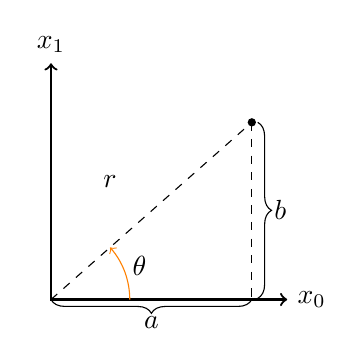
\begin{tikzpicture}[scale=1.5,decoration={brace,amplitude=5pt}]
    % Draw axes
    \draw [<->,thick] (0,2) node (yaxis) [above] {$x_1$}
        |- (2,0) node (xaxis) [right] {$x_0$};
    % Draw two intersecting lines
    %\draw (0,0) coordinate (a_1) -- (2,1.8) coordinate (a_2);
    \draw[dashed] (0,0)--(1.7,1.5);
    \node (r) at (.5,1) {$r$};
    %\draw (0,1.5) coordinate (b_1) -- (2.5,0) coordinate (b_2);
    % Calculate the intersection of the lines a_1 -- a_2 and b_1 -- b_2
    % and store the coordinate in c.
    %\coordinate (c) at (intersection of a_1--a_2 and b_1--b_2);
    \coordinate (c) at (1.7,1.5) ;
    \coordinate (b) at (0,0);
    \coordinate (a) at (1.5,0);
    \draw    pic["$\theta$", draw=orange, ->, angle eccentricity=1.2, angle radius=1cm]
    {angle=a--b--c};
    \draw [dashed,color=black] (1.7,1.5) -- (1.7,0)
    node [midway,anchor=west,inner sep=1pt, outer sep=5pt]{};
    \draw [decorate,color=black] (1.75,1.5) -- (1.75,.01)
   node [midway,anchor=west,inner sep=1pt, outer sep=5pt]{$b$};
    \draw [decorate,color=black] (1.7,0) -- (0,0)
   node [midway,anchor=north,inner sep=1pt, outer sep=5pt]{$a$};
    \fill[black] (c) circle (1pt) ;%node (point) [right] {$(a,b)$};
    % Draw lines indicating intersection with y and x axis. Here we use
    % the perpendicular coordinate system
    %\draw[dashed] (yaxis |- c) node[left] {$y'$}
    %    -| (xaxis -| c) node[below] {$x'$};
    % Draw a dot to indicate intersection point
\end{tikzpicture}
\end{document}
